%\documentclass[3p, sort&compress, 12pt]{elsarticle}
\documentclass[12pt, sort&compress]{report}
%\documentclass{article}
% Package
%==============================================
\usepackage{amsmath}
\usepackage{graphicx}
\usepackage[left=3.5cm, right=2.5cm, top=2cm, bottom=2cm,]{geometry}
\usepackage[bitstream-charter]{mathdesign}
\usepackage[utf8]{vietnam}
\usepackage{url}
\usepackage{hyperref}
\hypersetup{
	colorlinks=true,
	linkcolor=blue,
	filecolor=magenta,      
	urlcolor=Sepia,
}
\usepackage{ulem}
\usepackage{multicol}
\usepackage[table, dvipsnames]{xcolor}
\usepackage{array}
\usepackage{amsthm}
\usepackage[linesnumbered, ruled, longend]{algorithm2e}
\usepackage{subcaption}
\usepackage{caption}
\newcolumntype{P}{>{\centering\arraybackslash}p}
\newcolumntype{T}{>{\raggedleft\arraybackslash}p}
\usepackage{enumitem}
\usepackage{setspace}
\usepackage[noadjust,compress]{cite}
\usepackage{booktabs}
\usepackage{titlesec}

\titleformat*{\subsubsection}{\fontsize{14pt}{\baselineskip}\selectfont\bfseries}
%==============================================
\setlength{\parindent}{0pt}
\setlength{\parskip}{10pt}
\setitemize{topsep=3pt,parsep=0pt,itemsep=3pt,leftmargin=*,labelsep=10pt,align=parleft}
%==============================================
%\pgfpagesuselayout{boxed}
\begin{document}
\captionsenglish
\dateUSenglish
\begin{titlepage}
	% \fontfamily{cmr}\selectfont
	\begin{center}
		\vspace{1pt}
		{\textbf{\Large{HANOI UNIVERSITY OF SCIENCE AND TECHNOLOGY}}}\\[2cm]
		
	\end{center}
	\vspace{10pt}
	\begin{center}
		\vspace{8pt}
		\fontsize{34pt}{18pt}\selectfont 
		\textbf{\textrm{BACHELOR THESIS}} 
		\vspace{8pt}
	\end{center}
	\begin{center}
		\fontsize{21pt}{17pt}\selectfont 
		\textbf{\Large \textrm{The proposed Dual Encoder model for Open-domain question answering system: Case study in Vietnamese COVID-19 topics}} \\[1.5cm]
	\end{center}
	
	\begin{center}
		\fontsize{17pt}{17pt}\selectfont
		\textbf{\Large LE VU LOI}    \\
		loi.lv173240@sis.hust.edu.vn \\
		Talented class of Computer Science \\[0.5cm]
		\textbf{Information Technology} \\
		% \textbf{Chuyên ngành Khoa học máy tính} \\
		[1.5cm]
	\end{center}
	\vspace{1cm}
	\begin{table}[h!]
		\fontsize{14.5pt}{17pt}\selectfont
		\centering
		\begin{tabular}{ l} 
			\textbf{Supervisor:} Assoc. Prof. Pham Van Hai \hspace{0.6cm} \underline{\hspace{3.8cm}} \\ 
			\hspace{10cm}{\small Signature}\\
			Department of Information System \\[0.2cm]
			School of Information and Communications Technology \\ [5cm] 
		\end{tabular}
	\end{table} 
	
	\begin{center}
		\textbf{\large Hanoi, 6/2021}
	\end{center}
\end{titlepage}
\newpage

\begin{center}
	\noindent {\LARGE \textbf{Graduation mission ticket}}\\
\end{center}
\addcontentsline{toc}{chapter}{Graduation mission ticket}
\section*{Student information}

\begin{multicols}{2}
	\begin{itemize}
		\item \textbf{Fullname:} LE VU LOI
		\item \textbf{Telephone::} 098138986
		\item \textbf{Class:} Talented class of Computer Science
		\item \textbf{Email:} loi.lv173240@sis.hust\\.edu.vn
		\item \textbf{Program:} Talented Programs
	\end{itemize}
\end{multicols}
\begin{itemize}
	\item \textbf{Duration:} From February 2021 to June 2021.
\end{itemize}
\section*{Main purpose of the Thesis}
% Mục đích của đồ án là đề xuất phương pháp ứng dụng rừng ngẫu nhiên trong bài toán sinh ảnh với mô hình GANs nhằm tăng tính ổn định khi huấn luyện, tạo được một rừng các cây với lượng tri thức khác nhau cũng như cải thiện chất lượng ảnh được sinh ra. Nội dung của đồ án đó là phân tích chi tiết về lý thuyết và xem xét, đánh giá sự hiệu quả của phương pháp đề xuất trong thực nghiệm.
Main purpose of this Thesis is to propose to improve existing results on Open-domain question answering problem by training a Dual Encoder model with new objective, i.e. define a new loss function called \textit{stratified loss}, and to conduct a case study of Open-domain question answering system for Vietnamese COVID-19 data. 

\section*{Specific mission of the Thesis}
% Các nhiệm vụ cụ thể của đồ án bao gồm: Tìm hiểu về mô hình sinh, đặc biệt là mô hình GANs. Đề xuất một phương pháp nhằm cải thiện độ ổn định khi huấn luyện, tạo ra một rừng các cây với lượng tri thức khác nhau và cải thiện chất lượng ảnh sinh ra. Đưa ra chứng minh thực nghiệm về sự hiệu quả của phương pháp đề xuất.
\par Specific missions of the Thesis includes:
\begin{itemize}
	\item Study Open-domain question answering problem, especially the dense retriever component of the problem.
	\item Train and evaluate large models used in Open-domain question answering with large data on Cloud TPUs, reduce significant time for produce experimental results on the studied problem.
	\item Propose to use new objective called \textit{stratified loss} for training a Dual Encoder model for Open-domain question answering system.
	\item Conduct experiments to prove the effectiveness of proposed method.
	\item Conduct a case study of Open-domain question answering system for Vietnamese COVID-19 data.
\end{itemize}
\newpage
\section*{Pledge of student}
I am Le Vu Loi guarantee that this Thesis is my own work under the supervision of Associate Professor Pham Van Hai. \\
The results in this thesis are authentic and original.

%\restoregeometry
\begin{minipage}{0.5\textwidth}
	\hspace{1pt}
\end{minipage}
\begin{minipage}[t]{0.5\textwidth}
	
	\begin{center}
		\textit{Hanoi}, \today \\
		Author of thesis\\[3cm]
		
		Le Vu Loi
	\end{center}
\end{minipage}
\subsection*{Confirmation for the completeness of the thesis and permission for the thesis to be defense from supervisor:}
.\dotfill \\
.\dotfill \\ 
.\dotfill \\ 
.\dotfill \\
\begin{minipage}{0.5\textwidth}
	\hspace{1pt}
\end{minipage}
\begin{minipage}[t]{0.5\textwidth}
	
	\begin{center}
		\textit{Hanoi}, \today \\
		Supervisor\\[3cm]
		
		\textit{Assoc. Prof. Pham Van Hai}
	\end{center}
\end{minipage}
%==============================================
\newpage
\chapter*{Acknowledgment}
\addcontentsline{toc}{chapter}{Acknowledgment}
I want to express my sincere gratitude first to my supervisor Assoc. Prof. Pham Van Hai, who carefully guided me during the period of working on this Thesis. I'll have to thank Prof. Hai for all the patience, carefulness and enthusiastic he spent to me.
\par Secondly, I want to send millions thanks to my parents, my family for all the support they gave me. Without such a great spiritual motivation, I could not have surpassed the tough time during working on the Thesis.
\par Third, I am very grateful for being taught by lecturers at SoICT of HUST as well as all lecturers that have taught me. They are all great people that I can learn so much from.
\par Finally, I want thank all my friends, my classmates. I received a lot of help from them, not only during the period of this Thesis but also throughout 4 years I learned and worked at Hanoi University of Science and Technology.
%==============================================
\newpage
\chapter*{Summary of the Thesis}
\addcontentsline{toc}{chapter}{Summary of the Thesis}
This Thesis studied the problem of building Open-domain question answering system. An open-domain question answering system takes as input a user question in human language and produce a short, exact answer that user expects. Such a system is highly expected because it can significantly reduce the task of searching and reading documents usually performed by human. Based on existing methods in the literature, this Thesis implemented a pipeline of Dual Encoder and Cross Encoder architecture for Open-domain question answering system, efficiently training and evaluating the model on Cloud TPUs. After that, the Thesis proposed a \textit{stratified loss} to train the Dual Encoder model that finally resulted in an improvement in accuracy. As a case study, the Thesis trained a model for Vietnamese language with COVID-19 dataset. Numerous experiments were conducted to analyze effectiveness the proposed stratified loss and several initial results on the COVID-19 dataset were presented.
\par The organization of the Thesis is as follows:
\begin{itemize}
	\item Chapter I. Introduction: Overview about Open-domain question answering problem.
	\item Chapter II. Theoretical Preliminaries: Present theoretical prelininaries needed for the work of the Thesis.
	\item Chapter III. A pipeline of Dual Encoder and Cross Encoder for building Open-domain question answering system: Present in depth the Dual Encoder and Cross Encoder architecture of the system, the proposed \textit{stratified loss} and a use case for Vietnamese open-domain question answering system in COVID-19 topic.
	\item Chapter IV. Experimental results: Describe datasets, metrics, analysis and discuss on experimental results.
	\item Chapter V. Conclusion and Future works: Conclude the Thesis and outline several possible future directions.
\end{itemize}
%==============================================
\tableofcontents
%
\newpage
\renewcommand{\arraystretch}{1.25}
\chapter*{List of abbreviations}
\addcontentsline{toc}{chapter}{List of abbreviations}
\begin{table}[!htbp]
\caption{List of abbreviations}
\centering\begin{tabular}{p{.3\linewidth}p{.7\linewidth}}
	\toprule
	\textbf{Abbreviation} & \textbf{Explanation} \\
	\midrule
	QA & Question answering \\
	NLP & Natural Language Processing \\
	CNNs & Convolutional Neural Networks \\
	RNNs & Recurrent Neural Networks \\
	ODQA & Open-domain question answering \\
	LSTM & Long Short Term Memory \\
	GRU & Gated Recurrent Unit \\
	BERT & Bidirectional Encoder Representations from Transformers \\
	MRC & Machine Reading Comprehension \\
	\bottomrule
	\bottomrule
\end{tabular}
\label{table:0}
\end{table}
\listoffigures
\addcontentsline{toc}{chapter}{List of Figures}
\listoftables
\addcontentsline{toc}{chapter}{List of Tables}
%==============================================
\chapter{Introduction}
\label{chap:01}
\section{Overview}
\label{sec:1.1}
Question answering (QA) is at the medium level of difficulty among various tasks in Natural Language Processing (NLP). This task aims at giving the precise answer to a question given by human. An artificial agent with the capability of question answering is a direct evidence of computer understanding human language, which is the objective of research in NLP. Applications of question answering cover a wide range of domains, such as medical, bank, education, sales, etc. Actually, any service provider can benefit their customers by providing them with an automatic consultant whose core component is a question answerer. QA task is closely related to the task of dialogue system management, which is another challenging task in NLP. It makes sense to think of question answering as a step towards dialogue system management, since the former focuses on single-turn conversation and the latter deals with multi-turn one. Building efficient QA system lies in the middle of the journey to bring machine the ability of fully understanding human language.
\par Question answering can be classified into closed-domain and open-domain types. Closed-domain means that we need to provide the system with a question and the context containing the answer to that question. The system in this case is in charged of extracting the correct answer from the context, which is also known as machine reading comprehension. In contrast, Open-domain QA (ODQA) tries to find the answer without knowing about the context. ODQA is apparently more challenging than closed-domain one. To be able to answer open-domain questions, the system must either memorize knowledge in its internal structure or access to some information source to find information about the answer. Research about ODQA dated back to the 1960s \cite{green1961baseball}. In these early days, the main method was transforming the question into some form of query statements, then searching for relevant documents in a pre-constructed data source using lookup table \cite{green1961baseball} or syntactic pattern matching \cite{kupiec1993murax}. Starting in 1992, the Text REtrieval Conference (TREC) has significantly pushed the research on ODQA, especially in the aspect of information retrieval. According to the TREC-8 question answering track report \cite{voorhees1999trec}, most of participants used the following strategy. First, the input question was classified by its question word, i.e. "how", "what", "who", "why", "when", "where". The system then retrieved a set of documents using standard textual information retrieval method. Based on type of the question, which was determined in the first step, the system parsed the returned documents to get expected answer. Since this strategy is very intuitive, it turns out to become the choice of many later works on ODQA. In recent decades, deep learning or neural networks has extraordinarily boosted research in artificial intelligence (AI). Computer vision and Natural Language Processing are two fields that are the most benifited from this. As a critical task in NLP, ODQA has also moved towards the neural nets era. In 2017, D. Chen et. al proposed a retriever – reader architecture for reading Wikipedia to answer open-domain questions \cite{chen2017reading}. This work has drawn a huge attention of research community and promoted a large number of subsequent publications on ODQA \cite{wang2017rtheta3,asai2019learning,lee2019latent,min2019discrete,min2019knowledge,seo2019real,wang2019multi,guu2020realm,izacard2020leveraging,karpukhin2020dense,lewis2020retrieval,mao2020generation,min2020ambigqa,roberts2020much,xiong2020progressively,mao2021reader}. 
\par Motivated by the active research in ODQA, this Bachelor Thesis attempted to propose to improve existing results on ODQA. Furthermore, the Thesis also conducted a case study of ODQA for Vietnamese COVID-19 data. A demo web interface was also provided to illustrate results from ODQA system.
%focuses on building a retriever – reader architecture for ODQA task and then providing a case study in Vietnamese language. A demo web application is also provided to examine performance of the system.
\section{Problem formulation}
\label{sec:1.2}
This section provides definition of the Open-domain question answering task. This task is formulated as the followings:
\par\textbf{Input:}
\begin{itemize}
	\item A question in human natural language.
\end{itemize}
\hspace*{10pt} \textit{E.g.} Who is the founder of Google?
\par\textbf{Output:}
\begin{itemize}
	\item A list of answers for the input question.
\end{itemize}
\hspace*{10pt} \textit{E.g.} [Larry Page, Sergey Brin]
\par\textbf{Constraints:}
\begin{itemize}
	\item The system answers only factoid question. Factoid means that the question is about a fact and often can be answered with a short phrase. Yes/no questions, muliple-choice questions and reasoning questions are not factoid.\\[5pt]
	\textit{E.g.}
	\begin{itemize}
		\item Factoid question: What is the capital of Vietnam?
		\item Reasoning question: If 3 cats can catch 3 mice in 3 minutes, how many mices 	can 6 cats catch in 6 minutes?
	\end{itemize}
\end{itemize}
An ideal ODQA is expected to be able to answer any type of questions. To achieve that goal, however, is very challenging and often requires to build a complex system, which makes the system difficult to deploy into real applications. Besides, it makes more sense to build a system holding the facts about world, not a system that helps us solve math. Many questions even do not have an answer, like “Why does Nam hate Long?”. Answering more complex questions other than factoid questions were covered in other research, but is out of scope of this work.
\section{Thesis contribution}
\label{sec:1.3}
The contributions of this Bachelor Thesis is as following:
\begin{itemize}
	\item Propose to improve accuracy of Open-domain question answering system using \textit{stratified loss}.
	\item Conduct a case study for Open-domain question answering system in Vietnamese language for COVID-19 topic.
	%\item Provide a dataset for training an open-domain question answering system for COVID-19 topic.
	\item Build a web interface to illustrate results from Open-domain question answering system.
\end{itemize}
\par The remaining of this Thesis is organized as follows: chapter~\ref{chap:02} shows theoretical preliminaries needed for the work presented in this Thesis. Chapter~\ref{chap:03} is the main part of this Thesis, which presents in depth the architecture of Open-domain question answering system and proposal to improve the system performance by using \textit{stratified loss} to train a Dual Encoder model. Method for building an ODQA system for Vietnamese COVID-19 data is also provided in this chaper. Experiment results and analysis are provided in chapter~\ref{chap:04}. Finally, conclusion and futures are discussed in chapter~\ref{chap:06}.
%===================================================================
\chapter{Theoretical preliminaries}
\label{chap:02}
This chapter presents theoretical preliminaries needed for the work of this Thesis, including concepts in Deep Learning and Natural Language Processing.
\section{Neural Networks}
\label{sec:2.1}
Neural Networks or Deep learning is getting more and more robust for solving many tasks in computer science, especially in Computer Vision and Natural Language Processing (NLP). The building block of neural network is neuron. Neuron in the field of deep learning is inspired by biological neuron in human brain. Figure~\ref{fig:2:01} illustrates a neuron along with its components. In short, a biological neuron receives multiple input signals and produce an output if the aggregation of the input signals is greater than some threshold. 
\begin{figure}[!htbp]
	\centering
	\includegraphics[scale=.25]{images/biological_neuron.png}
	\caption{Biological neuron. Source: \cite{saurabh2021}}
	\label{fig:2:01}
\end{figure}
\par Artificial neuron has the same mechanism as biological neurons. They take as input  some variables, aggregate these variables in some way (normally taking the weighted sum), pass the output through an activation function and produce the final result (Figure~\ref{fig:2:02}).
\begin{figure}[!htbp]
	\centering
	\includegraphics[scale=0.4]{images/activation.jpg}
	\caption{Computation of an artificial neuron. Source: \cite{online}}
	\label{fig:2:02}
\end{figure}
\par A neural network is composed of multiple neurons connecting together, often organized in layer fashion. Since neural network is a computation model, its inputs must be represented in numbers (usually real numbers). Those numbers are fed into the network layer by layer to produce the final output. Figure~\ref{fig:2:03} gives an example of a neural network. Spefically, this neural network consists of 3 layers: input layer (in green), which is actually the numbers given as input of the network; hidden layer (in red), which take care of neural network computation and output layer (in yellow), which is what the network produces.
\begin{figure}[!htbp]
	\centering
	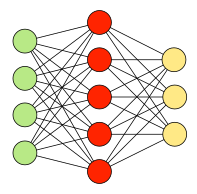
\includegraphics[scale=1.]{images/PDF/neural-net/neural-net.pdf}
	\caption{A simple neural network}
	\label{fig:2:03}
\end{figure}
\par What a neural network actually does is mapping the inputs to the expected outputs. Neural network is designed specially for learning the mapping function from available data. It reduces the tedious task of feature engineering. You just give the network the raw input, no need to worry about what features of the input should be selected to produce output, and then the neural network takes care of the whole process. It is like a magic black box that can give solution to many problems.
\par Up to now, there have been tons of different types of neural networks being proposed to solve different problems. Although neural network is very robust, it is not trivial to make it work on a specific problem. What data scientists are currently doing is to design good architecture for neural network for various tasks and problems. There are two main classes of neural networks, which are Convolution Neural Networks (CNNs) and Recurrent Neural Networks. The former was invented for the image processing tasks and the latter was original used for natural language processing.
\section{Language Model}
\label{sec:2.2}
Language model is a model that predicts some unseen words based on a given context. For example, given an incomplete sentence and predict the next word (Figure~\ref{fig:add:01:a}). Another example is predict  some masked words in a sentece (Figure~\ref{fig:add:01:b}). Language model is very important in the field of NLP since many downstream tasks like named entity recognition, question answering, part-of-speech tagger, etc. need to use it. By correctly predicting unseen words, language model can be considered as understanding the human natural language. Building a language model thus becomes the starting point  when researching in NLP. Types of language model includes statistical language model and deep language model (language model using neural network).  Along with the development of neural networks, deep language model has also gained many promise results and gradually become the replacement for most of traditional statistical models. It takes time to train a language model to understand human language, often measured in days or weeks. In 2018, Google released a fancy language model called BERT, which then has been used extensively by the research community as well as in production.
\begin{figure}[!htbp]
	\begin{subfigure}{.5\linewidth}
		\centering
		\includegraphics[scale=1.]{images/PDF/langModel/nextWord.pdf}
		\caption{}
		\label{fig:add:01:a}
	\end{subfigure}
	\begin{subfigure}{.5\linewidth}
		\centering
		\includegraphics[scale=1.]{images/PDF/langModel/maskedWord.pdf}
		\caption{}
		\label{fig:add:01:b}
	\end{subfigure}
	\caption{Language modeling examples: (a) next word prediction; (b) masked word prediction}
	\label{fig:add:01}
\end{figure}
\section{Transformers}
\label{2.3}
In the early days of deep learning in NLP, a very common neural network architecture called Recurrent Neural Networks (RNNs) was proposed and used extensively for various NLP problems. The idea of RNNs is using a shared weights across all input words to learn the contextual representation of words. This idea successfully worked and quickly became default choice for solving many NLP tasks. However, it has several drawbacks: (1) it processes the input words sequentially so parallel computing cannot be utilized to speed up training; (2) since it used shared weights for all input words, the gradient signals when performing backward propagation must go through a very long path, causing to gradient vanishing and gradient exploding. The latter problem was addressed by two architectures named Long-Short Term Memory (LSTM) and Gated Recurrent Units (GRU), which create a “highway” for gradient signal to properly flow into every part of the network. However, problem of unable to parallelize remained. In 2017, transformers architecture was introduced in \cite{vaswani2017attention} and then marked a milestone in NLP. This new architecture addressed all previous problems and produced much better results than the existing baselines. Figure~\ref{fig:2:04} describes the architecture of transformers. In essence, it is a sequence-to-sequence model containing two parts: encoder and decoder. The encoder encodes the input sentence into a sequence of vectors in hidden space. The decoder then uses these vectors to produce outputs. Different from RNNs, which compacts the contextual information into a word by sequentially process each word of the sentence from left to right or right to left, transformers uses a mechanism called attention, where each word in the sentence directly attends to all other words. Thus, it avoids the gradient vanishing or gradient exploding problem (there is no long path when flowing gradient signals backward) and can capture contextual information of words that are far apart.
\begin{figure}[!htbp]
	\centering
	\includegraphics[scale=.7]{images/transformers.png}
	\caption{Transformers architecture. Source: \cite{vaswani2017attention}}
	\label{fig:2:04}
\end{figure}
\par Attention mechanism is described as follows. A query $Q$ needs to know which items are important in a list of given items, where each item is represented as a key $K$ and a value $V$. To know that, it computes the similarity scores between $Q$ and each key $K$. How to compute the similarity scores is not restricted. The common choice is dot product or bi-linear function. The similarity scores are then normalized into a probability vector called attention scores, where each value of the attention scores is the importance of the corresponding item. As the last step, $Q$ takes the weighted sum of all values $V$ with respect to the probability vector and get the output as its new representation. The above process is mathematically formulated as belows:
\par \textbf{Input}
\begin{itemize}
	\item $Q \in \mathbb{R}^{q \times d}, K \in \mathbb{R}^{n \times d}, V \in \mathbb{R}^{n \times d}$, where $q$ is the number of queries, $n$ is the number of items, $d$ is the size of query, key and value vectors.
\end{itemize}
\par \textbf{Computation}
\begin{itemize}
	\item Similarity scores: $S = QK^T \in \mathbb{R}^{q \times n}$
	\item Attention scores: $\mathbb{\alpha} = \text{softmax}(S) \in \mathbb{R}^{q \times n}$
\end{itemize}
\par \textbf{Output}
\begin{itemize}
	\item $\tilde{Q} = \mathbb{\alpha}V \in \mathbb{R}^{q \times d}$, the new representation of $Q$.
\end{itemize}
\par Encoder and decoder components of transformers are built by stacking multiple encoder or decoder blocks on top each other. Each block in turn composes of several layers. There are two types of layers in transformers architecture, which are feed-forward layer and multihead attention layer. Multihead attention is basically the same as the abovementioned attention mechanism, but uses attention multiple times and then concatenates the output together. The encoder is responsible for transforming the input sentence, which is in human language, to vectors in a vector space. The output vectors of encoder are expected to hold the contextual information of input words (the contextual information is captured by multihead self-attention layer). In the decoder side, output words are generated sequentially. A special [START] token is first fed into  decoder, then goes through a series of decoder blocks, each contains a \textbf{masked multihead attention} layer, a normal multihead attention layer with keys and values taken from encoder outputs, and a feed-forward layer. On top of all decoder block is a softmax classifier which produces the probability of the next word. The word with highest probability is chosen as next word and this next word is then concatenated with previously produced words to create input for the next feed forward through decoder. The decoding process stops when a [END] token appears. Here, we have the concept of masked multihead attention layer. During training decoder, we want each word to attend only the words preceeded it. Hence, we mask out the subsequent words by setting attention scores for those words to zeros. 
\par The original transformers applied to Neural Machine Translation task, but in general in can be used in any sequence-to-sequence task such as text summarization, question answering,… After transformers was released, there were appearances of many fancy modern deep language models. These language models either based on encoder or decoder components of transformers. Typical examples are BERT (encoder-based) and T5 (decoder-based). The next section discusses about BERT, which stands for Bidirectional Encoder Representations from Transformers, released by Google in 2018 \cite{devlin2018bert}.
\section{BERT - The state-of-the-art pretrained language model}
\label{2.4}
\begin{figure}[!htbp]
	\centering
	\includegraphics[scale=.6]{images/bert.png}
	\caption{BERT architecture. Source: \cite{bert}}
	\label{fig:2:05}
\end{figure}
\par In recent years, NLP community has seen the word “BERT” ubiquitously. BERT is a language model trained on two tasks: masked language modeling and next sentence prediction. BERT architecture is the same as encoder of transformers (Figure~\ref{fig:2:05}). In essence, it encodes the input sentence into a sequence of word vectors, where each word vector holds the contextual information of the corresponding word. These contextual word vectors were proved to significantly boost many downstream tasks in NLP. By learning to correctly predict the masked words and the next sentence, BERT model achieves ability to understand human language. Currently, there have a variety of high-quality pretrained language models, but BERT is a good candidate for starting researching in the field of NLP.
%===================================================================
\newpage
\chapter{The proposed Dual Encoder model for Open-domain question answering system: Case study in Vietnamese COVID-19 topics}
\label{chap:03}
%This chapter presents method for building an open-domain question answering system, including system pipeline design, data preparation and core components' training process.  
%This chapter first presents method for building an general open-domain question answering system, including system pipeline design, data preparation and core components' details. The second-half part of this chapter presents an use case of building question answering system for answering COVID-19 question in Vietnamese.
This chapter first presents high-level architecture of an Open-domain question answering system, then dives into details of each component in the system including dense retriever (Dual Encoder) and extractive reader (Cross encoder). After that, the proposed method for improving dense retriever (Dual Encoder) component is presented. The last section of this chapter considers a case study of Open-domain question answering system for Vietnamese COVID-19 data.
\section{Open-domain question answering system pipeline}
\label{sec:3.1}
Standing from a non-tech user's point of view, a computer that has the ability of question answering should take as input a human-language question (through typing text or through speech) and produces the answer to the user (also in form of human language). This is exactly what an open-domain question answering is. Another type of question answering system is closed-domain. In this type of system, computer is provided with a context to search for answer alongside input question. Closed-domain question answering is known with a more popular name, which is Machine Reading Comprehension (MRC). MRC problem has been studied for a long time and it is a core component of Open-domain question answering system. Since there is no context provided to the open-domain question answering system, it must retrieve contexts itself based solely on the input question. Look up information for a question and then figure out the answer seems not to be so complicated to human but is very challenging for computer. To perform this task, an open-domain question answering system usually contains two components: a retriever to get relevant contexts for an input question, and a reader to produce answer from the retrieved contexts. Almost modern open-domain question answering system follows this retriever-reader pipeline. Figure~\ref{fig:01} is an illustration of this pipeline. 
\begin{figure}[!htbp]
	\centering
	\includegraphics[scale=.8]{images/PDF/overall_arch/architecture.pdf}
	\caption{Retriever - reader pipeline of Open-domain question answering system}
	\label{fig:01}
\end{figure}
\par There are many different ways of how to retrieve and how to read. Traditional retriever often get relevant contexts based on keyword overlapping between question and contexts. A well-known algorithm for this type of search is TF-IDF or BM25. This search method is also known as sparse vector searching because questions and contexts are represented by a vector with many zeros. Prior to nowadays' deep learning era, BM25 was the most popular method not only for open-domain question answering, but also for a broader field in computer science which is information retrieval. In recent years, with the development of neural network, a.k.a deep learning and hardware accelerators like GPUs and TPUs, many problems have been addressed by adopting modern neural network model. Specific to open-domain question answering problem, sparse retriever is now replaced by dense retriever, in which question and contexts are encoded to a low-dimension vector space and there is no longer redundant zeros.
\par On the side of reader, the most common used types are extractive reader and generative reader. Different from retriever, reader does not have a long time of development and both extractive and generative types are based on recent neural network models. Given a question and several contexts (the results of retriever component), extractive reader tries to extract the answer by predicting the start token and end token of the answer inside these contexts (Figure~\ref{fig:02}). In contrast, generative reader is not restricted to produce answers that are contained in contexts but can freely generate any answers. As shown in Figure~\ref{fig:03}, the phrase "Maths teacher" does not appear in the context, but is the right answer for the input question. Intuitively, generative reader is more challenging than extractive one since there is no constraint about the output answers. Actually, generative model needs to learn more than extractive model to get the expected results. This thus lead to the challenge of bigger model size and longer training time. 
\begin{figure}[!htbp]
	\centering
	\includegraphics[scale=1.0]{images/PDF/extractive_reader/extractive_reader.pdf}
	\caption{Extractive reader}
	\label{fig:02}
\end{figure}
\begin{figure}
	\centering
	\includegraphics[scale=1.0]{images/PDF/generative_reader/generative_reader.pdf}
	\caption{Generative reader}
	\label{fig:03}
\end{figure}
This Thesis studies extractive reader and dense retriever. Dense retriever was shown to better than sparse retriever in existing research \cite{karpukhin2020dense}. In general, neural networks are now performing much better than traditional methods. However, traditional information retrieval method like BM25 is helpful for generating training data for dense retriever. %How to generate training data with BM25 is later presented in section.
Although results returned by BM25 are not always exact, it can significantly reduce time used for manually tagging data since it provides annotator with several potential choices. Later, annotator can decide whether or not to use the results of BM25.
\section{Dual encoder and cross encoder architecture of Open-domain question answering system}
\label{sec:3.2}
As aforementioned, open-domain question answering system includes two core components, which are retriever and reader. Retriever and reader implemented in this Thesis are dense retriever and extractive reader, in which dense retriever follows dual encoder architecture and extractive reader follows cross encoder architecture. The generative reader mentioned in previous section is also a robust model that can produce answers that are not constrained to be contained in any contexts, but it comes at the cost of huge model size and requiring much more time for training model to converge. Studying about generative reader might be considered in future works of this Thesis.
%This section provides details of model architecture as well as training process for each component.
\subsection{Dense retriever}
\label{sec:3.2.1}
Retriever model used in this Thesis is based on dense retriever model proposed in \cite{karpukhin2020dense}. From the base model, this Thesis has proposed to use \textit{stratified loss} function to improve model's accuracy. Details about retriever model are presented in the following sections.
\subsubsection{Model architecture}
\label{sec:3.2.1.1}
Dense retriever follows dual encoder architecture which contains two neural networks, which are question encoder and context encoder. Each encoder can be any type of neural network that take as input a text sequence and produce a sequence of embedding vectors for that sequence. How dense retriever works is illustrated in Figure~\ref{fig:04}.
\begin{figure}[!htbp]
	\centering
	\includegraphics[scale=.8]{images/PDF/biencoder/biencoder.pdf}
	\caption{Dense retriever pipeline}
	\label{fig:04}
\end{figure}
\par As shown in Figure~\ref{fig:04}, work flow of dense retriever contains two phases. Offline phase takes long time to complete but we only need to do this once. In this phase, we need a data source which contains large number of contexts. Each context goes through the context encoder and output an embedding vector. These embedding vectors are then indexed using faiss indexer \cite{JDH17}, in which faiss is an efficient approximate similarity search algorithm that can scale to billion vectors. In the online phase, system receives the input question and encodes that question to an embedding vector using question encoder. Next, this question embedding vector is fed to faiss indexer to perform $k$-nearest neighbor search. The final output of the online phase is top $k$ most relevant contexts to the input question, which then further be fed to the reader to produce the final answer.
\subsubsection{Training retriever}
\label{sec:3.2.1.2}
To train the dense retriever, this Thesis simultaneously trained the context encoder and the question encoder. Subsequent sections presents details of the training process.
\par \textit{a) Training data}
\par Each training sample contains the followings:
\begin{itemize}
	\item 1 question;
	\item 1 positive context, which is the context that has answer for the question;
	\item $m$ negative contexts, which do not contain answer for the question;
\end{itemize}
An example of a training sample will look like Figure~\ref{fig:05}.
\begin{figure}[!htbp]
	\centering
	\includegraphics[scale=.8]{images/PDF/retriever_sample/retriever_sample.pdf}
	\caption{Retriever training sample. Blue text is answer for the sample's question.}
	\label{fig:05}
\end{figure}
\par \textit{b) Loss function}
\par Let $\mathbb{E}_Q$, $\mathbb{E}_C$ be the question encoder and context encoder respectively. Let $D_i = \left\langle q_i, p_i^+, \left\{p^-_{i,j}\right\}_{j=1}^m\right\rangle$ be the i-th training sample, where:
\begin{itemize}
	\item $q_i$: the question;
	\item $p_i^+$: the positive context;
	\item $\left\{p_{i, j}^-\right\}_{i=1}^m$: $m$ negative contexts
\end{itemize}
\par After forwarding $D_i$ to the retriever, we will get:
\begin{itemize}[itemsep=5pt]
	\item $qe_i = \mathbb{E}_Q(q_i)$: embedding vector of the input question;
	\item $pe_i^+ = \mathbb{E}_C(p_i)$: embedding vector of the positive context;
	\item $pe_{i,j}^- = \mathbb{E_C}(p_{i,j}^-), \: j = \overline{1, m}$: embedding vectors of $m$ negative contexts.
\end{itemize}
\par Objective of training retriever is to maximize similarity between $qe_i$ and $pe^+_i$ while minimizing similarity between $qe_i$ and $pe_{i,j}^-, \: j=\overline{1, m}$. Similarity score can be calculated using any metrics. But to serve the purpose of later indexing using faiss algorithm, the metric should be one of L2 norm, cosin and dot product. These metrics are supported by faiss. To obtain the training objective, we use negative log likelihood loss function as below:
\begin{equation}
	\label{eq:01}
	\mathcal{L}_i = -\log\left\{\dfrac{\exp\left[{\text{sim}\left(qe_i, pe_i^+\right)}\right]}{\exp\left[{\text{sim}\left(qe_i, pe_i^+\right)}\right] + \sum\limits_{j=1}^m\exp\left[\text{sim}\left(qe_i, pe_{i,j}^-\right)\right]}\right\}
\end{equation},
where \textit{sim} is the similarity function.
\par Here, $\mathcal{L}_i$ is the loss value over the i-th training sample. Suppose we have $n$ training samples, the loss value over the training dataset is average of loss value over each training sample:
\begin{equation}
	\mathcal{L} = \dfrac{1}{n}\mathcal{L}_i
\end{equation}
\subsection{Extractive Reader}
\label{sec:3.2.2}
A reader, or a machine reader, is one that can read a set of documents and output the answer. While retriever "skims through" a huge amount of documents to get a much smaller document subset, reader "swallows" a small amount of documents to produce the exact answer. In case of extractive reader, if number of documents to be read is greater than 1, reader needs to perform 2 tasks: re-ranking and reading. Re-ranking means selecting the best document out of the documents retrieved by the retriever. Each document after re-ranking has a re-rank/selection score and the document with the highest score is selected. Reading or extracting is to find the start and end position of the answer inside the selected document. The work of re-ranking and reading can be implemented using a common neural networks or two seperate ones. To avoid confusing, let single-document reader be used to refer to the reader that reads only one document at a time. This Thesis uses two different neural networks for the re-ranker and the single-document reader. Computational cost of re-ranker is much more expensive than single-document reader since re-ranker operates on a set of documents while single-document reader only needs to operate on a single one. Hence, seperating re-ranking and reading work has the advantage of training the single-doc reader with more data during training re-ranker. Beside, we can flexibly use different neural networks architecture for these two components. 
\subsubsection{Model architecture}
\label{sec:3.2.2.1}
\textit{a) Re-ranker}
\par The task performed by re-ranker is quite similar to what is done by retriever. Both re-ranker and retriever assigns some similarity score to the document with respect to the input question. The difference is at the scope where retriever and re-ranker work. Since retriever deals with huge amount of documents, it does not need to thoroughly look into each single document but only acts as a simple filter. The task of actually reading each single document is left to the extractive reader, which contains re-ranker and single-document reader. In the literature, there are two neural architectures used to compute similarity between input question and documents. The first is known as dual encoder or bi-encoder, which is the architecture of previously presented retriever. The second is called cross encoder, which is usually used for the reader (all types of reader, including re-ranker, single-document reader and generative reader). Figure~\ref{fig:06} shows the difference of the two architectures. 
\begin{figure}[!htbp]
	\begin{subfigure}{\linewidth}
		\centering
		\includegraphics[scale=.9]{images/PDF/compare_arch/dual_encoder.pdf}
		\caption{}
		\label{fig:06:a}
	\end{subfigure}
	\begin{subfigure}{\linewidth}
		\centering
		\includegraphics[scale=.9]{images/PDF/compare_arch/cross_encoder.pdf}
		\caption{}
		\label{fig:06:b}
	\end{subfigure}
	\caption{Dual encoder and cross encoder architecture: (a) Dual encoder; (b) Cross encoder}
	\label{fig:06}
\end{figure}
\par Re-ranker used in this Thesis follows cross encoder architecture. As shown in Figure~\ref{fig:06:b}, cross encoder jointly encode question and context into one single embedding vector. Given a question and $n$ contexts, we concatenates the question to each context, adds special {\sffamily [CLS]} and {\sffamily [SEP]} tokens and then feed each concatenated sequence to the re-ranker. At the output, we have $n$ jointly question-context embedding vectors. These vectors then go through a softmax classifier to produce a probability vector. The context that has the highest probability is finally chosen as the best context (the context that is the most likely to have the answer). Figure~\ref{fig:07} is the full picture of re-ranker. Mathematically, computation of re-ranker happens as follows:
\begin{itemize}
	\item Input:
	\begin{itemize}
		\item $\mathbf{X} \in \mathbb{R}^{K \times L \times d}$: $K$ input sequences, each of which is the concatenation of the question and a context. Each token of a sequence is represented by vector in $\mathbb{R}^d$. Here, $d$ is the embedding vector size and $L$ is length of input sequence.
	\end{itemize}
	\item Joint question-context embedding vector of i-th input sequence $\mathbf{X}_i$ ($\mathbf{X}_i \in \mathbb{R}^{L \times d}$):
	\begin{itemize}
		\item $\mathbf{H}_i = crossEncoder\left(\mathbf{X}_i\right) \in \mathbb{R}^{L \times d}$
		\item $\mathbf{E}_i = pooled\left(\mathbf{H}_i\right) \in \mathbb{R}^d$. \\\textit{pooled} is a function that take as input a sequence of vectors and return a single one. Popular pooling function is max pooling, mean pooling, averaging pooling, .etc. Since cross encoder allows each token in the input sequence to interact with all others, a more powerful pooling operator is using directly {\sf [CLS]} token. Embedding vector corresponding to this token is also the embedding vector of the whole sequence.
	\end{itemize}
	\item Projecting to scalar value:
	\begin{itemize}
		\item $\alpha_i = \mathbf{E}_i^T\mathbf{w} \in \mathbb{R}$: scalar value corresponding to the i-th input sequence. The higher this value is, the more relevant the question and the context are.
	\end{itemize}
	\item Softmax function: Let $\alpha = \left(\alpha_1, \alpha_2, ..., \alpha_K\right) \in \mathbb{R}^K$, then:
	\begin{itemize}
		\item $\tilde{\alpha} = \text{softmax}\left(\alpha\right) \in [0, 1]^K$: probability distribution over $K$ input contexts.
	\end{itemize}
\end{itemize}
\begin{figure}[!htbp]
	\centering
	\includegraphics[scale=.6]{images/PDF/full-reranker/fullRerank.pdf}	
	\caption{Model architecture for re-ranker}
	\label{fig:07}
\end{figure}
\par \textit{b) Single-document reader}
\par Single-document reader also uses cross encoder architecture. Cross encoder architecture is very suitable for single-document reader since it deals with the interaction among tokens in a sequence, i.e. every token in question and context interacts with each other. These interactions cannot be captured directly in dual encoder architecture. Most part of single-document reader is the same as re-ranker. The difference is that single-document reader produce two probability distributions, one for predicting answer's start position and one for predicting answer's end position, while re-ranker produces one probability distribution for predicting the best context. Figure~\ref{fig:08} shows the detailed architecture of the single-document reader. It looks a bit different from Figure~\ref{fig:07} and Figure~\ref{fig:06:b} because there is an extra \textit{token embeddings} block. This turns out to be no different at all. Since re-ranker only considers the embedding vector of the whole question-context sequence, token embeddings part is hide for saving space.
\begin{figure}[!htbp]
	\centering
	\includegraphics[scale=.7]{images/PDF/singleDocReader/singleDocReader.pdf}
	\caption{Single-document architecture}
	\label{fig:08}
\end{figure}
\par Computation flow of single-document reader is described as follows:
\begin{itemize}
	\item Input
	\begin{itemize}
		\item $\mathbf{X} \in \mathbb{R}^{L \times d}$: A sequence of length $L$ composed of question token embeddings and context token embeddings. Each embedding vector has size $d$.
	\end{itemize}
	\item Forwarding through cross encoder
	\begin{itemize}
		\item $\mathbf{H} = crossEncoder\left(\mathbf{X}\right) \in \mathbb{R}^{L \times d}$
	\end{itemize}
	\item Project to scalar value
	\begin{itemize}
		\item $\alpha = \mathbf{H}.\mathbf{w}_s \in \mathbb{R}^{L}$, where $\mathbf{w}_s \in \mathbb{R}^{d \times 1}$
		\item $\beta = \mathbf{H}.\mathbf{w}_e \in \mathbb{R}^{L}$, where $\mathbf{w}_e \in \mathbb{R}^{d \times 1}$
	\end{itemize}
	\item Softmax function
	\begin{itemize}
		\item $\tilde{\alpha} = \text{softmax}(\alpha)$: probability distribution of being start token.
		\item $\tilde{\beta} = \text{softmax}(\beta)$: probability distribution of being end token.
	\end{itemize}
\end{itemize}
\subsubsection{Training reader}
\label{sec:3.2.2.2}
\par \textit{a) Training re-ranker}
\par \textit{Training data}
\par Training data for re-ranker is described as follows:
\begin{itemize}
	\item 
	$\mathcal{G} = \left\{\left\langle q_i, p_i^+, \left\{p_{i, j}\right\}_{j=1}^n\right\rangle\right\}_{i=1}^m$: dataset containing $m$ training samples, in which:
	\begin{itemize}
		\item $q_i$: i-th input question
		\item $p_i^+$: i-th positive context
		\item $\left\{p_{i,j}\right\}_{j=1}^n$: $n$ negative contexts in the i-th training sample.
	\end{itemize}
\end{itemize}
\par \textit{Loss function}
\par Loss function used to train re-ranker is negative-log likelihood. Re-ranker tries to maximize the probability of the positive context over all input contexts. 
\begin{itemize}
	\item Assumptions
	\begin{itemize}
		\item $e_i^+$: joint question-context embedding vector of i-th input question and i-th positive context produced by cross encoder.
		\item $\left\{e_{i, j}^-\right\}_{j=1}^n$: $n$ joint question-context embedding vectors of i-th input question and $n$ corresponding negative contexts of this input question. 
	\end{itemize}
	\item Loss formula \\[10pt]
	\begin{equation}
		\label{eq:04}
		\mathcal{L}_i =-\log\left\{ \dfrac{\exp\left[\text{sim}\left(e^+_i\mathbf{w}\right)\right]}{\exp\left[\text{sim}\left(e^+_i\mathbf{w}\right)\right] + \sum\limits_{j=1}^n\exp\left[\text{sim}\left(e^-_{i,j}\mathbf{w}\right)\right]}\right\}
	\end{equation}
\end{itemize}
\par \textit{b) Single-document reader}
\par \textit{Training data}
\begin{itemize}
	\item $\mathcal{H} = \left\{ L_i, s_i, e_i\right\}_{i=1}^{m}$: dataset containg $m$ samples, in which:
	\begin{itemize}
		\item $L_i$: concatenation of a question and a positive context (context that has answer).
		\item $s_i$: start position of the answer in the concatenated sequence $L_i$
		\item $e_i$: end position of the answer in the concatenated sequence $L_i$
	\end{itemize}
\end{itemize}
\par \textit{Loss function}
\begin{itemize}
	\item Assumptions
	\begin{itemize}
		\item $h_i$: joint question-context embedding vector produced by cross encoder.
		\item $\alpha_i$: probability distribution of being the start token.
		\item $\beta_i$: probability distribution of being the end token.
	\end{itemize}
	\item Loss formula 
	\begin{equation}\label{eq:06}\mathcal{L}_i = -\log\alpha_i[s_i] - \log\beta_i[e_i]\end{equation}
\end{itemize}
Note that this loss function contains two parts. The first part is the negative log-likelihood loss for the start token and the second is also negative log-likelihood loss but for end token. Loss formula in equation~\eqref{eq:06} means that the model will try to maximize probability of joint probability of $s_i$ being the start token and $e_i$ being the end token.
\section{Proposed method for training Dual Encoder with stratified loss}
\par To efficiently train the retriever using loss function defined~\eqref{eq:01}, Karpukhin et. al \cite{karpukhin2020dense} proposed to use the in-batch strategy, in which negative contexts of a training sample are taken from positive context of other samples in the same batch. Thus, each forward to the retriever model requires much less data than normally using seperate negative contexts for each training sample. Alongside this in-batch strategy, the authors use another type of negative context called hard negative context. Hard negative contexts do not contain answer for the input question but are very similar to the positive one. These hard negative contexts are often obtained by using another algorithm like BM25 or the retriever model in the previous epoch of training process. Using hard negative contexts and in-batch loss were shown to be very efficient and those are the keys to the success of dense retriever model. Karpukhin et. al used one hard negative context per a sample and they pointed out that using 2 or more hard negative contexts did not improve the results (using 2 hard negative contexts was even worse). However, a closer look into the model shows that dense retriever can easily distinguish between positive context and non-relevant negative contexts, but has difficulty distinguishing positive context and hard negative ones. Thus, this Thesis propose a loss function called \textit{stratified loss} which can help the model better learning the difference between positive and hard negative contexts.
\par The idea of stratified loss function is simple. It is sum of two loss functions, where each is a negative log likelihood loss as presented above. The difference between these two loss functions is that the first is designed to learn to differentiate between positive and hard negative contexts, while the second learns to differentiate between hard negative and normal negative ones. The consequence of using stratified loss is that the model will learn to know which context is more negative. In contrast, the original loss function treats all negative contexts the same. Mathematically, stratified loss is computed as followings:
\par\textit{Inputs}:
\begin{itemize}
	\item A batch $\mathcal{D}$ of $b$ training samples. Here, embedding vectors are used instead of raw text input since loss function only applies to embedding vectors (state differently, loss calculation is performed after forwarding raw text input through retriever model). Each sample $\mathcal{D}_i, \:i = \overline{1, b}$ contains:
	\begin{itemize}
		\item $q_i$: question embedding;
		\item $p_i^+$: positive context embedding;
		\item $p_{i,j}^-,\: j=\overline{1, w}$: $w$ hard negative context embeddings.
	\end{itemize} 
\end{itemize}
\par\textit{Loss formula}:
\begin{equation}
	\begin{array}{ll}
		\label{eq:03}
		\mathcal{L}_i = &-\log\left\{\dfrac{\exp\left[{\text{sim}\left(q_i, p_i^+\right)}\right]}{\exp\left[{\text{sim}\left(q_i, p_i^+\right)}\right] + \sum\limits_{j=1}^w\exp\left[\text{sim}\left(q_i, p_{i,j}^-\right)\right]}\right\} \\[40pt]
		&-\sum\limits_{j=1}^w\log\left\{\dfrac{\exp\left[\text{sim}\left(q_i, p_{i,j}^-\right)\right]}{\exp\left[\text{sim}\left(q_i, p_{i,j}^-\right)\right] + \sum\limits_{k\in \{1, 2,..., b\}\backslash\{i\}} \exp\left[\text{sim}\left(q_i, p_k^+\right)\right]}\right\}
	\end{array}
\end{equation}
\par The first term of equation~\eqref{eq:03} is written exactly the same as in equation~\eqref{eq:01}, but note that hard negative contexts are used instead of normal negative ones. The second term is what stratified loss differs from the original loss, which makes retriever give higher similarity score (with respect to the input question) to hard negative contexts than normal negative ones. This loss formula is taken over a batch of input samples, not a single one. The benefit is each single sample contains only positive and hard negative contexts while normal negative contexts are taken from other positive contexts in the same batch. 
\section{Building Vietnamese question answering system for COVID-19 topic}
\label{sec:3.3}
This section present an use case of open-domain question answering system for COVID-19 topic in Vietnamese language. To build Vietnamese question answering system for COVID-19 topic, the first thing to do is preparing dataset. Currently, there is no publicly avaible dataset specifically built for open-domain question answering for COVID-19 topic. Hence, following sections will show the details about the process of crawling, annotating and preparing a COVID-19 dataset.
\subsection{Data crawling}
\label{3.3.1}
To build open-domain question answering system, the first thing is to build a data source. Data source or context source is where retriever looks for information to answer question. It should be large enough to cover almost information required by users. As one of the largest data source on the Internet, Wikipedia contains millions of articles, cover information about any thing in the world. Since data about COVID-19 is restrict in a narrow domain, it is likely that several thousands of contexts can cover everything in the domain.
\par 
%\par Retrieving large amount of data requires
\par This Thesis targeted to build a data source that contains about 150,000 contexts. Although these large amount of contexts are not required to cover everything about COVID-19 topic, this large amount challenge the system and thus we can measure how well the system perform. Usually, text documents are not simply a sequence of continuous words. They are organized into sections, subsections, etc., has highlight or emphasize part. These structures contains rich information about the document. To capture some of these structure information, each document used to train open-domain question answering system is represented as the concatenation of document title and document content.
\par
\par This Thesis focused on crawling COVID-19 data. The remain contexts in the data source can be about any domain, just need to be large enough to challenge the system. A common data source that one might think of is Wikipedia. However, the pattern of data in Wikipedia is very different from data related to COVID-19 topic, thus might be too easy for the system. Hence, this Thesis used context source in medical domain, in which COVID-19 is a sub-domain. In total, this Thesis crawled 168,388 contexts.
%Since crawling data source is not the focus of this Thesis, as well as this work is very time consuming, the data source is taken from Social Data Lab of CIST Institute of CMC Corporation, in which the author of this Thesis currently works. These data are taken with permission and is not publicly available. It is used only in the scope of this Thesis.
\par COVID-19 data was crawled using {\tt requests-html} library of python, which is a library capable of retrieve dynamic javascript content of web pages. Data is crawled from several Vietnamese medical websites but mainly from \url{https://suckhoecongdong.net.vn/}.
\par Raw html content is first processed by removing html tag using regular expression. Regular expression is also used to capture headings or sections of the crawled article. Since the retriever and reader is a neural network based on BERT-architecture, which can process up to 512 tokens in a sequence, crawled article must be break into several smaller passages. Specifically, each passage must have number of single word inside the range (70, 120).
\par MySQL database is used to store data. In total, there have been 1470 passages that are stored in MySQL database. Storaging data in database is more beneficial than just using normal files because we can easily perform CRUD operators using database. 
\par An example of crawled COVID-19 data is given in Figure~\ref{fig:09}. As shown in this figure, each context source has title (the second column) and content (the third column). Usually, several contexts has the same title, since these contexts come from one single article on the Internet. 
\begin{figure}
	\centering
	\includegraphics[scale=.5]{images/crawled_data.png}
	\caption{Example of a context}
	\label{fig:09}
\end{figure}
\subsection{Data annotating}
\label{sec:3.3.2}
Training data for open-domain question answering system needs to be annotated. Data for training an open-domain question answering system should contain the following fields:
\begin{itemize}
	\item {\sf question}: a human-language question
	\item {\sf answers}: a list of answers corresponding to the question
	\item {\sf positive contexts}: a list of contexts that contains at least one of the answers
	\item {\sf hard negative contexts}: a list of contexts that related to the question, i.e. has the same keywords as the question, mention the same thing as in the question, .etc, but not contain the answer.
\end{itemize}
Intuitively, more positive contexts and more hard negative contexts is better for training the system. But using more of these contexts results in significantly increasing training time while may not be really necessary. Beside, the job of annotating data is very time consuming. Hence, only one positive and one hard negative is annotated per an input question. 
\par Each training sample is annotated as follows. Given a context, which is one of the crawled context from data crawling phase, we need to make a question based on this context, satisfying that answer for that question is contained with the context. This context is then consider as positive context for the question. After making question and extract answers from positive context, the next thing is to make a hard negative context. Hard negative context usually mentions the same object as in positive context but does not provide information to answer the question. For example, when an user asks "Number of new COVID-19 cases in Hanoi today", positive context exactly mention this information, while hard negative context may talk about "number of new COVID-19 cases in Ho Chi Minh city". Choosing hard negative context is totally dependant on the annotator and is the most time consuming part of annotating data.
\par To efficiently annotate data, this Thesis uses {\tt django}, which is a python web framework. This framework provide an easy way for CRUD data in web interface. Figure~\ref{fig:10} shows the web interface for annotating data.
\begin{figure}[!htbp]
	\centering
	\includegraphics[scale=.3]{images/annotate.png}
	\caption{Annotating data web interface using {\tt django}}
	\label{fig:10}
\end{figure}
There are several rules applied for annotating data as follows:
\begin{itemize}
	\item At least one of answers to the question must be contained in positive context;
	\item A single answer to a question should not be longer than 10 single words;
	\item Length of hard negative context in single words should be in the range (70, 150);
	\item Avoid yes/no question
	\item Avoid question that requires reasoning
\end{itemize}
Note that the open-domain question answering considered in this Thesis is targeted at answering factoid question. The reader component of the system is extractive reader, which is not suitable for answering question that requires reasoning. Since yes/no question also requires reasoning, we try to avoid this type of question. Usually, answer for a factoid question is short, and the design of extractive reader does not perform well for long answer. Other rules are already mentioned in previous sections.
\par In the final, we have total of 630 training samples. 
\subsection{Training the system on annotated data}
\label{sec:3.3.3}
Training open-domain question answering system for Vietnamese COVID-19 dataset follows the architectures and processes presented in section~\ref{sec:3.2.1} and section~\ref{sec:3.2.2}. For pretrained Vietnamese language model, this Thesis used {\tt NlpHUST/vibert4news-base-cased} from \href{https://huggingface.co/}{\tt huggingface}. For Vietnamese, there are also another well-known pretrained language model, which is {\tt PhoBERT} \cite{nguyen2020phobert}
%===================================================================
\chapter{Experimental results}
\label{chap:04}
This chapter focuses on conducting experiments on dense retriever. All experiments are conducted using Natural Question dataset \cite{kwiatkowski2019natural}. The built Vietnamese COVID-19 dataset mentioned in the previous section serves as an use case of applying open-domain question answering in real life. This dataset is still small and has not been thoroughly experimented. For the extractive reader, this Thesis tries to reproduce the bench mark results in the literature following the existing architecture and configurations. 
\section{Datasets}
\label{sec:4.1}
\subsection{Natural Question}
\label{sec:4.1.1}
Natural question is a dataset provided by Google. This dataset contains real user queries issued to the google search engine \cite{kwiatkowski2019natural}. Natural Question contains annotated data for answering both long answer and short answer, where short answer is the exact phrase that represents the answer, and long answer is the smallest HTML bounding box that contains all information required to answer the question. In total, there are 307,373 training samples, 7,830 development samples and 7,842 test samples. Each sample contains a question, a context corresponding to that question. start position and end position of long and short answers inside that context. 
\par Natural Question is built specifically for question answering problem. Context source of Natural Question dataset is from Wikipedia. This Thesis doest not perform processing Natural Question dataset from the beginning, but use a pre-processed data provided by \cite{karpukhin2020dense}. A training sample for dense retriever of this processed dataset look like Figure~\ref{fig:11}.
\begin{figure}[!htbp]
	\centering
	\includegraphics[scale=1.]{images/PDF/retriever_sample/nq_sample.pdf}
	\caption{Natural Question training data sample for dense retriever}
	\label{fig:11}
\end{figure} 
\par As shown in Figure~\ref{fig:11}, each training samples has a question, a list of answers, a list of positive contexts, a list of negative contexts and a list of hard negative contexts. Each context has a title and a text content. According to \cite{karpukhin2020dense}, each context has 100 single words, retrieved by non-overlapping breaking an Wikipedia article into small contexts. In the end, the processed dataset contains 58,880 training samples, 8,757 development samples and  3,610 test samples. For the context source, there is totally 21,015,324 contexts.
\subsection{Vietnamese COVID-19 dataset}
\label{sec:4.1.2}
This section recap some features of the built Vietnamese COVID-19 dataset. This dataset contains 630 training samples. The development and test set have not been built yet. Each training sample contains a question, a list of answers to that question, a positive context and a hard negative context. Compare to Natural Question dataset, COVID-19 dataset is much smaller. However, COVID-19 dataset serves as an use case of open-domain question answering system when applying to Vietnamese language. In the aspect of application, this dataset can completely be used to build a well-performed system. But in the research aspect, this dataset needs to be improved and expanded. 
%===================================================================
\section{Metrics}
\label{sec:4.2}
\subsection{Top-$k$ hits score}
\label{sec:4.2.1}
The most popular metrics to measure the performance of dense retriever is top-$k$ hits. The dense retriever gets a top-$k$ hit if at least one of $k$ contexts returned by it contains answer for the input question. 
\subsection{Exact match}
\label{sec:4.2.2}
To estimate performance of extractive reader as well as end-to-end system, exact match metrics is used. As the name suggests, the system get one exact match hit if the answer returned by the system matches exactly one of the true answers. 
\section{Experimental settings}
\label{sec:4.3}
\subsection{Environment settings}
\label{sec:4.3.1}
All experiments are conducted using Google Cloud TPUs and Google Compute Engine. Table~\ref{tab:01} gives details about these devices.
\renewcommand{\arraystretch}{1.25}
\begin{table}[!htbp]
	\caption{Devices for running experiments}
	\label{tab:01}
	\centering
	\begin{tabular}{|l|l|}
		\hline
		Cloud TPUs & VM Compute Engine \\\hline
		\begin{minipage}{6cm}
			TPU v3-8 on-demand:
			\begin{itemize}
				\item TPU version 3
				\item 8 TPU cores
				\item 16GiB memory / TPU core
			\end{itemize}
		\end{minipage} & \begin{minipage}{6cm}
			\begin{itemize}\item OS: Ubuntu 20.04  \item Disk: 30GB \item RAM: 16GB \item nCPUs: 4\end{itemize}
		\end{minipage} \\\hline
	\end{tabular}
\end{table}
\par TPUs are very beneficial for training huge data. It is much faster than using several GPUs simultaneously. As reported in \cite{karpukhin2020dense}, the author used eight 32GB GPUs for training model, 50 2-gpu nodes for inference (generating embedding vectors for 21 millions contexts) and a server with Intel Xeon CPU E5-2698 v4
@ 2.20GHz and 512GB memory for indexing and retrieving embedding vectors. These are a huge computational resources that seems impossible for one to have. This Thesis successfully reproduce the training and inference process on Cloud TPUs. Price for hiring a TPU v3-8 on-demand on Google Cloud is 8\$ USD/hour. This is much cheaper than hiring GPUs, but still a very high price. Luckily, Google offers a TPU Research Cloud (TRC) program with access to 5 TPU v3-8 on-demand, 5 TPU v2-8 on-demand and 100 preemptible TPU v2-8. Details about types of Cloud TPUs is available at \url{https://cloud.google.com/tpu/}. Also, user of Google Colab can access Cloud TPUs as well but for a very limited time (less than 12 hours).
\par Training and inference of the system is implemented using {\tt Tensorflow 2.4.1}. which is one of the most well-known framework for Deep Learning. Using tensorflow is the best way to run code on Cloud TPU. Both tensorflow and Cloud TPUs are owned by Google. Hence, they are designed for working best together.
%===================================================================
\subsection{Data settings}
\label{sec:4.3.2}
Testing performance of dense retriever requires huge amount of time. We need to generate embedding vectors for all 21 millions contexts in the data source, which takes 40 minutes on 50 2-GPUs node \cite{karpukhin2020dense}. This is unrealistic for one to build and test an open-domain question answering system. Hence, this Thesis only uses a subset of context source to test the performance of dense retriever. Specifically, all contexts that contains answers for question in test set must be included in the new subset. Since there are a number of question in the test set that do not have a corresponding positive context in the context source, we need to add additional contexts to the new subset. These additional contexts are manually annotated by searching Wikipedia for the correct answer of a question. Additional contexts guarantee that the maximum accuracy of the model is 100\%, which is necessary for comparing different models. If the context source does not contain positive contexts for some question, we cannot know how well retriever perform on that question and thus, not fair for comparing models.
\par There are about 450 out of 3610 questions in the test set do not have corresponding positive context in the context source. This Thesis uses 700,000 out of 21 millions contexts as the new context source. Along with 450 annotated contexts, the new context source contains about 700,450 contexts.
\par The training data is left unchanged. Dense retriever was trained on full training data, which take several minutes on each epoch.
\section{Experimental results on dense retriever}
\label{sec:4.4}
This section provides analysis on effect of different parameters to the performance of dense retriever. There are several default parameters used consistently throughout this section. Table~\ref{tab:02} shows values of these parameters. The meaning of each parameter is as follows:
\begin{itemize}
	\item {\tt pretrained language model}: the pretrained language model used to initilize the question encoder and context encoder of dense retriever.
	\item {\tt tokenizer}: the tokenizer used to tokenize question and contexts into tokens and the convert each token to a token id.
	\item {\tt adam-eps, adam-betas}: hyperparameters for Adam optimizer. Refer to \cite{kingma2014adam} to get details about this optimizer.
	\item {\tt max context length}: max length of each context counting in single words. Each context is truncated and padded before being trained.
	\item {\tt epochs}: number of times the whole training dataset is iterated through
\end{itemize}
\begin{table}[!htbp]
	\caption{Default parameter settings}
	\label{tab:02}
	\centering
	\begin{tabular}{p{.4\linewidth}p{.4\linewidth}}
		\hline
		{\tt pretrained language model}  & {\tt bert-base-uncased} \\\hline
		{\tt tokenizer} & {\tt bert-base-uncased} \\\hline
		{\tt adam-eps} & {\tt1e-8} \\\hline
		{\tt adam-betas} & {\tt (0.9, 0.999)} \\\hline
		{\tt max context length} & {\tt 256} \\\hline
		{\tt epochs} & {\tt 40} \\\hline
	\end{tabular}
\end{table}
\subsection{Effects of different loss functions}
\label{sec:4.4.1}
Before coming up with the proposed stratified loss, the author of this Thesis has done extensively experiments on a set of different loss functions to find out which is the best. This section provide a thorough analysis on effect of different loss functions.
\par First, let define several loss functions. These loss functions contains:
\begin{table}
	\caption{List of loss functions}
	\label{tab:03}
	\centering
	\begin{tabular}{p{.3\linewidth}p{.6\linewidth}}
		\hline
		{\tt inbatch} & which is the original loss function, defined in equation~\eqref{eq:01} \\\hline
		{\tt threeLevel} & try to distinguish between positive and hard negative contexts, between positive and normal negatives, between hard negatives and normal negatives, using a mix of binary cross entropy and negative log-likelihood. \\\hline
		{\tt twolevel} & try to distinguish between positive and hard negative contexts, and between positive and normal negative contexts, using only negative log-likelihood.\\\hline
		{\tt hardnegvsneg} & try to distinguish between positive and hard negative contexts, between hard negatives and normal negatives, using a mix of binary cross entropy and negative log-likelihood.\\\hline
		{\tt hardnegvsnegsoftmax} & try to distinguish between positive and hard negatives, between hard negatives and normal negatives, using only negative log-likelihood.\\\hline
		{\tt threelevelsoftmax} & try to distinguish between positive and hard negatives, between positive and normal negatives, between hard negatives and normal negatives, using only negative log-likelihood.\\\hline
		
	\end{tabular}
\end{table}
\par The proposed \textit{stratified loss} mentioned in \ref{chap:03} In short, all these loss functions involve three types of context: positive, hard negative and normal negative. There is only one positive context but multiple hard negative and normal negative ones. Assume $\alpha$ is the similarity score between input question and positive context, $\left\{\beta_i\right\}_{i=1}^x$ are similarity scores between input question and $x$ hard negative contexts and $\left\{\gamma_j\right\}_{j=1}^y$ are similarity scores between input question and $y$ normal negative contexts. Followings are the loss formula defined between each two types of contexts:
\begin{itemize}
	\item Loss defined on positive and hard negatives (softmax)
	\begin{equation}
		\label{eq:07}
		\mathcal{L}_{\text{posVsHard}} = -\log\dfrac{\exp\left(\alpha\right)}{\exp\left(\alpha\right) + \sum\limits_{i=1}^x\beta_i}
	\end{equation}
	\item Loss defined on positive and normal negatives (softmax)
	\begin{equation}
		\label{eq:08}
		\mathcal{L}_{\text{posVsNeg}} = -\log\dfrac{\exp\left(\alpha\right)}{\exp\left(\alpha\right) + \sum\limits_{i=1}^x\gamma_i}
	\end{equation}
	\item Loss defined on hard negatives and normal negatives
	\begin{itemize}
		\item Binary cross entropy:
		\begin{equation}
			\label{eq:09}
			\begin{array}{l}
				\tilde{\beta} = \text{softmax}(\beta) \\
				\tilde{\gamma} = \text{softmax}(\gamma) \\ 
				l = (1, 1, ..., 1, 0, 0, ... ,0, 0),\:\: \text{ where } x \text{ first values are 1 and } y \text{ remaining values are 0 } \\
				c = l / \sum\limits_{i=1}^{x + y} l \\
				\mathcal{L}_{\text{hardVsNeg}} = -\sum\limits_{i=1}^x c_i\log\left(\tilde{\beta_i}\right) - \sum\limits_{j=x+1}^{x+y}(1 - c_j)\log(1-\tilde{\gamma}_{j-x}),
			\end{array}
		\end{equation}
		\item Softmax
		\begin{equation}
			\label{eq:10}
			\mathcal{L}_{\text{hardVsNeg}} = -\log\sum\limits_{i=1}^x\dfrac{\exp\left(\beta_i\right)}{\exp\left(\beta_i\right) + \sum\limits_{j=1}^y\exp\left(\gamma_j\right)}
		\end{equation}
	\end{itemize}
\end{itemize}
\par Loss function used in~\eqref{eq:07}, ~\eqref{eq:08} and~\eqref{eq:10} are negative log-likelihood, which are the same as the loss function defined in equation~\eqref{eq:01}. In~\eqref{eq:09}, binary cross entropy loss is used. Binary cross entropy between a scalar $e$ and a scalar $f$, $e, f \in [0, 1]$ is defined as:
\begin{equation}
	\label{eq:11}
	\text{binaryCrossentropy}(e, f) = -e\log(f) - (1-e)\log(1-f)
\end{equation}
\par Assume $e$ is a predefined constant, this function has minimum at $f=e$. According to that, the function in~\eqref{eq:09} has its minimum at $\tilde{\beta}_i = c_{i}, \forall 1 \leq i \leq x$ and $\tilde{\gamma_j}=c_{j + x}, \forall 1\leq j\leq y$, meaning that hard negative contexts have higher similarity value than normal negative contexts. Both equation~\eqref{eq:09} and ~\eqref{eq:10} aim to give higher similarity score to hard negative contexts than to normal negative contexts. However, computation of~\eqref{eq:10} is more expensive.
\par Using combinations of~\eqref{eq:07}, ~\eqref{eq:08}, ~\eqref{eq:09}, ~\eqref{eq:10} give us the different losses as shown in Table~\ref{tab:03}.
%\par \textit{Compare between {\tt inbatch} and {\tt threeLevel} loss functions}
\subsubsection{Comparison between {\tt inbatch} and {\tt threeLevel} loss functions}
\label{sec:4.4.1.1}
Performance of dense retriever using {\tt inbatch} loss and {\tt threeLevel} loss are shown in Figure~\ref{fig:12}. This comparison is done using following configurations:
\begin{itemize}
	\item {\tt batch\_size=16}
	\item {\tt num\_hard\_negatives=8}
	\item {\tt max\_grad\_norm=2.0}
\end{itemize}
\par {\tt num\_hard\_negative} here is the number of hard negative contexts in each training sample. This parameter does not apply for {\tt inbatch} loss. For {\tt inbatch} loss, we always use 1 hard negative context for training. {\tt max\_grad\_norm} is used to clip gradient when computing backpropagation if the gradient value is to large. These three parameters are applied for all subsequent sections inside section~\ref{sec:4.4.1} if there is no explicit settings for these parameters.
\begin{figure}[!htbp]
	\centering
	\includegraphics[scale=.7]{images/PDF/experiments/inbatch_threelevel_4-1-1.pdf}
	\caption{Top-K hits when using inbatch and threelevel loss}
	\label{fig:12}
\end{figure}
\par We can see that {\tt threelevel} loss has higher top-k hits score than {\tt inbatch} when $k$ is small. For retriever, it is not too important to have high top-k hits score for small values of $K$ because those contexts retrieved by retriever are further feed to re-ranker, which takes the job of finding what context having the answer. The important thing is retriever can retrieve at least one positive context. However, this is not true if we use retriever independently from reader, i.e. if we use retrieve as a search engine, the answer should be contained in a few top contexts retrieved by the retriever. No matter which is more important: overall top-k hits scores, or top-k hits scores for small K, we can clearly see that {\tt inbatch} outperforms {\tt threelevel} loss in this case.% In this experiment scenario, dense retriever is trained for 40 epochs for both {\tt inbatch} and {\tt threelevel} loss using max question length 32. Later sections also analyze the effect of max query length parameter.
\subsubsection{Comparison between {\tt inbatch} and {\tt twolevel} loss functions}
\label{sec:4.4.1.2}
This experiments also has the same configuration as the previous: max question length 32, trained for 40epochs. Figure~\ref{fig:12} shows the comparison.
\begin{figure}[!htbp]
	\centering
	\includegraphics[scale=.7]{images/PDF/experiments/inbatch_twolevel_4-1-2.pdf}
	\caption{Top-K hits when using inbatch and twolevel loss}
	\label{fig:13}
\end{figure}
\par Actually, there is no significant difference between these two loss. The difference is {\tt inbatch} loss considers all contexts of other training samples in the same batch as the negative context, while {\tt twolevel} considers only positive contexts of other training samples from the sample batch. When we train retriever on large data for many epochs, top-K hits corresponding to these two loss tend to be similar. In Figure~\ref{fig:13}, we see only a small gap between twolevel and inbatch curve, which is expected for these two loss functions.
\subsubsection{Comparison between {\tt inbatch} and {\tt hardnegvsneg} loss functions}
\label{sec:4.4.1.3}
\begin{figure}[!htbp]
	\centering
	\includegraphics[scale=.7]{images/PDF/experiments/inbatch_hardnegvsneg_4-1-3.pdf}
	\caption{Top-K hits when using inbatch and hardnegvsneg loss}
	\label{fig:14}
\end{figure}
As shown in Figure~\ref{fig:14}, there is a big gap between top-K hits score between hardnegvsneg and inbatch loss. This phenomena is the same as the first scenario considered in \ref{sec:04:01:01}. At this point, we can see that using binary cross entropy loss is not efficient. This may be due to the essence of the function. In case of softmax, maximizing the probability of the positive also minimizing probability of all other negatives (because sum of the probability distribution is 1, and we are trying to assign probability 1 for the positive, whichs mean other negatives will receive the probability 0). In contrast, when using binary cross entropy, each probability is independently optimized. The fact that positive has high probability does not affect the probability of other negatives. We now remove {\tt hardnegvsneg} and {\tt threelevel} from consideration.
\subsubsection{Comparison between {\tt inbatch} and {\tt threelevelsoftmax} loss functions}
\label{sec:4.4.1.4}
\begin{figure}[!htbp]
	\centering
	\includegraphics[scale=.7]{images/PDF/experiments/inbatch_threelevelsoftmax_4-1-4.pdf}
	\caption{Top-K hits when using inbatch and threelevelsoftmax loss}
	\label{fig:15}
\end{figure}
Figure~\ref{fig:15} shows the consistently better top-K hits scores of {\tt threelevelsoftmax} over {\tt inbatch} loss. The gap between two curves at small values of K is remarkable. Using {\tt threelevelsoftmax}, we obtain both objective: high top-K hits score for small values of K and high top-K hits score over a wide range of K's values. Then, {\tt threelevelsoftmax} is better than {\tt inbatch} loss both in case used as search engine and in case used in combination with reader.
\subsubsection{Comparison between {\tt inbatch} and {\tt hardnegvsnegsoftmax} loss functions}
\label{sec:4.4.1.5}
The last loss function is considered in this section. Figure~\ref{fig:16} is the comparison between {\tt hardnegvsnegsoftmax} and {\tt inbatch}. This figure is almost the same as Figure~\ref{fig:15}, showing that using {\tt hardnegvsnegsoftmax} and {\tt threelevelsoftmax} give the same effect. However, using {\tt hardnegvsnegsoftmax} is cheaper since it only compute two types of loss.
\begin{figure}[!htbp]
	\centering
	\includegraphics[scale=.7]{images/PDF/experiments/inbatch_hardnegvsnegsoftmax_4-1-5.pdf}
	\caption{Top-K hits when using inbatch and threelevelsoftmax loss}
	\label{fig:16}
\end{figure}
\subsubsection{Comparison with Dense Passage Retriever model\cite{karpukhin2020dense}}
\label{sec:4.4.1.6}
This section compares Dense Passage Retriever (DPR) model with the best tuned model in this Thesis. Among current research on retriever, retriever model proposed by this work is one of the best model available. The author of Dense Passage Retriever shows that their dense retriever outperforms built-in search engine of Wikipedia. Figure~\ref{fig:17} shows the comparison between this Thesis's best model and the baseline model proposed in \cite{karpukhin2020dense}. Top-K hits score of the baseline model is produced using this Thesis's author code, which using Tensorflow and inference on Cloud TPUs. The original checkpoint is provided in PyTorch. The results produced by the Thesis's author code exactly match the results reported in github repository of the baseline model. (github repo only provides top-1, top-5, top-20 and top-100 hits). The checkpoint that is currently made publicly avaible is different from what is reported in original paper. There is an big improvements between the currently public model and the model reported originally. Table~\ref{tab:04} show the improvements of new DPR model.
\begin{figure}[!htbp]
	\centering
	\includegraphics[scale=.7]{images/PDF/experiments/benchmark_compare.pdf}
	\caption{Top-K hits when using baseline DPR model and best tuned model used in this Thesis}
	\label{fig:17}
\end{figure}
\begin{table}
	\caption{Top-K hits between original DPR model and new DPR model}
	\label{tab:04}
	\centering
	\begin{tabular}{lll}
		\hline
		Top-K contexts & Original DPR model & New DPR model \\\hline
		1 & 45.87 & 52.47 \\\hline
		5 & 68.14 & 72.24 \\\hline
		20 & 79.97 & 81.33 \\\hline
		100 & 85.87 & 87.29 \\\hline
	\end{tabular}
\end{table}
\par As shown in Figure~\ref{fig:17}, the baseline DPR model performs significantly better than the best tuned model when $K < 20$. When $K \geq 20$, the best tuned model starts to outperform the baseline model. As $K$ becomes greater, the gap between two curves is getting more clear.
\par Karpukhin et. al. pointed in \cite{karpukhin2020dense} that using 1 hard negative context significantly boost the model, but using more give no improvements or even worse. However, baseline DPR model uses {\tt inbatch} loss, which considers hard negative and normal negative context the same. As shown in Figure~\ref{fig:15} and ~\ref{fig:16}, taking the difference between hard negative and normal negative context into consideration gives consistently better results.
\par Note that this experiment is conducted on a subset of original context source (this experiments consider 700,450 contexts while the original context source contains 21,015,324 contexts). Then, the top-K hits score is slightly different. This difference is shown in Figure~\ref{fig:18}. From Figure~\ref{fig:17}, Table~\ref{tab:04} and Figure~\ref{fig:18}, we can deduce that best tune model is competitive with the original DPR with small K values and is significantly better for high values of $K$. Note that the improvements introduced by new DPR model compared to original DPR model is related to hard negative context. New DPR model was trained with hard negative contexts mined from an existing DPR model.
\par After thoroughly analysis performance of dense retriever using different loss functions as well as study existing results, we can see that hard negative contexts are the key for success of an efficient open-domain question answering system. Such efficient loss function like \textit{stratified loss} can nicely boost the retriever performance.
\begin{figure}
	\centering
	\includegraphics[scale=0.7]{images/PDF/experiments/700Kvs21M.pdf}
	\caption {Difference in top-K hits score when using 700,045 contexts and 21,015,324 contexts}
	\label{fig:18}
\end{figure}

\subsection{Effects of different question length}
\label{sec:4.4.2}
To efficiently train dense retriever on TPUs, each question is padding to the same length and each context is also padding to the same length. Since length of question is much smaller than length of context, we can pad question to a length that is smaller than the context padding length. In this experiment, two values of max question length are examined, which are 32 and 256. These values are power of 2 and such power of 2 is beneficial for TPUs to efficiently compute. Figure~\ref{fig:19} shows top-K hits scores when using the same configuration training retriever except for that max question length. As shown in this figure, question length 32 is competitive with question 256, sometimes even better. This implies that padding tokens to the input sequence does not affect the ability of the retriever model to learn. Hence, in the best tuned model, this Thesis uses the question length of 32 (note that this number is counted in tokens). 
\begin{figure}[!htbp]
	\begin{subfigure}{.5\linewidth}
		\centering
		\includegraphics[scale=0.45]{images/PDF/experiments/inbatch_batch64.pdf}
		\caption{}
		\label{fig:19:a}
	\end{subfigure}
	\begin{subfigure}{.5\linewidth}
		\centering
		\includegraphics[scale=.45]{images/PDF/experiments/twolevel_batch16.pdf}
		\caption{}
		\label{fig:19:b}
	\end{subfigure}
	\caption{Comparison of top-K hits scores using different question length: (a) Using {\tt inbatch} loss, {\tt batch\_size=64}; (b) Using {\tt twolevel} loss, {\tt batch\_size=16}}
	\label{fig:19}
\end{figure}

\subsection{Effects of using different poolers for getting the sequence embedding}
\label{sec:4.4.3}
Dense retriever, or BERT model in general, take as input a sequence of tokens, produces a sequence of token embeddings. To represent the whole sequence, we need to use a pooler operator over all tokens. There are several ways to do this: sum, average, max, .etc. Since BERT is a neural architecture that can capture direct interaction between every pair of tokens in the input sequence, we can use a "pooler" token to be the representation of the whole sentence. This is actually done very commonly. Before feeding the input sequence to BERT model, we append a special {\tt [CLS]} token at the beginning of the sequence. After forwarding through BERT, the embedding vector of this {\tt [CLS]} is used as embedding vector of the whole sequence. 
\par To give the model more flexibility to learn, embedding vector of {\tt [CLS]} token is further feed into a fully connected layer to produce the final embedding for the sequence. This type of pooler is actually implemented into some Deep Learning library as the default behavior. This Thesis also studies the effect of using fully connected layer on top of {\tt [CLS]} token embedding. The results is shown in Figure~\ref{fig:20}
\begin{figure}[!htbp]
	\begin{subfigure}{.5\linewidth}
		\centering
		\includegraphics[scale=.45]{images/PDF/experiments/poolerCompare_batch16.pdf}
		\caption{}
		\label{fig:20:a}
	\end{subfigure}
	\begin{subfigure}{.5\linewidth}
		\centering
		\includegraphics[scale=.45]{images/PDF/experiments/poolerCompare_batch64.pdf}
		\caption{}
		\label{fig:20:b}
	\end{subfigure}
	\caption{Comparison of top-K hits scores when using fully connected pooler and when not use: (a) Using {\tt inbatch} loss, {\tt batch\_size=16}; (b) Using {\tt inbatch} loss, {\tt batch\_size=64}}
	\label{fig:20}
\end{figure} 
\par Both Figure~\ref{fig:20:a} and Figure~\ref{fig:20:b} shows that using Fully Connected layer tears down top-K hits scores significantly. This might be due to the fact that weights of Fully Connected layer do not interact directly with the token embedding vectors. Fully Connected layer only transfer information contained in {\tt [CLS]} token to the final output. The job of transfering information might require large training steps to be successfully.
\subsection{Choosing best tuned model}
\label{sec:4.4.4}
After conducting many experiments, there are some highlight findings:
\begin{itemize}
	\item Using negative log-likelihood loss is better than binary cross entropy. Hence, {\tt threelevelsoftmax} and {\tt hardnegvsnegsoftmax} are chosen as the best loss functions. Since {\tt hardnegvsneg} offers cheaper computation, this {\tt hardnegvsnegsoftmax} is used for the best tuned model. {\tt hardnegvsnegsoftmax} is essentially the \textit{stratified loss} proposed in chapter\ref{chap:03}
	\item Using different question length does not affect performance of the model. Hence, the best tuned model uses the shortest question length possible. This length must be long enough to cover every question in the dataset. If too short, question will be truncated and thus lead to lost of information.
	\item Using fully connected layer on top of {\tt [CLS]} token embedding downgrades the model performance significantly. Hence, best tuned model doest not use this fully connected layer 
\end{itemize}
\par Beside these findings, a try to speed up training has also been done. Speed up is done by increase {\tt learning\_rate} and {\tt max\_grad\_norm}. While {\tt learning\_rate} does not help, increase {\tt max\_grad\_norm} results in a minor improvements.
\par To summary, Figure~\ref{fig:21} shows a bigger picture of the performance of dense retriever with all types of loss functions.
\begin{figure}
	\centering
	\includegraphics[scale=.7]{images/PDF/experiments/K_hits.pdf}
	\caption{Comparison of top-K hits scores using different loss functions}
	\label{fig:21}
\end{figure}
%%===================================================================
\section{Experimental results on extractive reader}
\label{sec:4.5}
Re-ranker and single-document reader have not been fully implemented in this Thesis. As an initial results on training single-document reader, this Thesis achieves exact match score of 56.6 on the Natural Question dataset (the preprocessed data set provided in \cite{karpukhin2020dense})
\section{Experimental results on Vietnamse COVID-19 dataset}
\label{sec:4.6}
This Thesis trained a dense retriever on COVID-19 dataset. Since the training samples is small (630 training sample), the model took only 1.4s on a TPU v3-8 to complete a train epoch. Dense retriever model for COVID-19 dataset was trained for 20 epochs with parameter settings be the same as used for training retriever on Natural Question dataset. The initial pretrained language model used is {\tt NlpHUST/vibert4news-base-cased} from \url{https://huggingface.co/}. 
\par Table~\ref{tab:05} is the complete list of parameters used to train this model.
\begin{table}
	\caption{Parameters used for training dense retriever on Vietnamese COVID-19 dataset}
	\label{tab:05}
	\centering
	{\tt
		\begin{tabular}{p{.4\linewidth}p{.5\linewidth}}
			\hline
			batch\_size & 8 \\\hline
			pretrained\_language\_model & NlpHUST/vibert4news-base-cased \\\hline
			learning\_rate & 2e-5 \\\hline
			epochs & 20 \\\hline
			loss function & inbatch \\\hline
			max\_context\_length & 256 \\\hline
			max\_query\_length & 64 \\\hline
			max\_grad\_norm & 3.0 \\\hline
	\end{tabular}}
\end{table}
\par Results from the model are shown in~\ref{fig:22} and Figure~\ref{fig:23}. As the results show, model retrieves very relevant contexts within first few retriever results.
\begin{figure}[!htbp]
	\centering
	\includegraphics[scale=.4]{images/vietnameseRetriever.png}
	\caption{Retriever results of dense retriever trained on COVID-19 dataset}
	\label{fig:22}
\end{figure}
\begin{figure}[!htbp]
	\centering
	\includegraphics[scale=.4]{images/covid19.png}
	\caption{Retriever results of dense retriever trained on COVID-19 dataset}
	\label{fig:23}
\end{figure}
%===================================================================
\chapter{Conclusion and future works}
\label{chap:06}
\section{Conclusion}
\label{sec:6.1}
%This Bachelor Thesis attempted to build an Vietnamese Open-domain question answering for COVID-19 topic. To successfully conduct an use case in Vietnamese language for COVID-19 data, the Thesis first studied on the basis of Open-domain question answerning system. After thoroughly diving into the architecture and detailed components of the system, this Thesis proposed to efficiently train the system using \textit{stratified loss} function. By conducting numerous experiments, the proposed loss function is shown to consistently outperform existing loss function used in the literature. Most of the Thesis's effort was to effectively implement the system using Cloud TPUs. By successfully making use of Cloud TPUs, the Thesis can conduct large number of experiments in short time, reduced the time for experiments from impossible to several hours. Being able to rapidly produce experimental results allows the Thesis to come up with the proposed \textit{stratified loss} function. After implementing and evaluating the open-domain question answering on bench mark dataset, this Thesis performed the job of building COVID-19 dataset. Data about COVID-19 topic was crawled from several medical articles and then was annotated using an easy web interface built with Django. A retriever model was built with this COVID-19 dataset and initial results of applying open-domain question answering system to COVID-19 dataset are quite positive.
This Bachelor Thesis attempted to improve accuracy of existing Open-domain question answering system. To achieve that goal, the Thesis first studied on the basis of Open-domain question answerning system, including surveying existing methods. After thoroughly diving into the architecture and detailed components of the system, this Thesis proposed to efficiently train a Dual Encoder model using \textit{stratified loss}. By conducting numerous experiments, the proposed method was shown to consistently outperform existing methods in the literature. Most of the Thesis's effort was to effectively implement the system using Cloud TPUs. By successfully making use of Cloud TPUs, the Thesis can conduct large number of experiments in short time, reduced the time for experiments from impossible to several hours. Being able to rapidly produce experimental results allowed the Thesis to fully understand what factors have effects to the model, then the Thesis can devise the new stratified loss function. After implementing and evaluating the open-domain question answering on bench mark dataset, this Thesis performed the job of building COVID-19 dataset. Data about COVID-19 topic was crawled from several medical websites and then was annotated using an easy web interface built with Django. A Dual Encoder model was built with this COVID-19 dataset and initial results of applying open-domain question answering system to COVID-19 data are quite positive.
\section{Future Works}
\label{sec:6.2}
There are many works that are left to successfully build an qualified Vietnamese open-domain question answering system. To build an real application, we need a pipeline from data crawling, data management, data annotating, model training and evaluation. In the research aspect, re-ranker and single-document reader model needs to be studied more in depth. Open-domain question has the potential to be applied to many domains and can tackle many business problems. For example, if the company wants to build a service that can automatically answer users with the question about the company itself, this is where OpenQA comes in. Following the open-domain question answering system pipeline and collect a dataset about the company, open-domain question answering will be likely to perform well for the required task. Open-domain question answering also relates to several other problems such as: information retrieval, machine reading comprehension, knowledge base construction, etc. Relation between open-domain QA and knowledge base/knowledge graph is a really interesting problem that have not been yet studied widely.
%====================================================================
\newpage
\bibliographystyle{unsrt}
\bibliography{reference}
\addcontentsline{toc}{chapter}{References}
\end{document}